\documentclass[11pt]{article}
\usepackage[margin=1in]{geometry} 
\usepackage{amsmath,amsthm,verbatim,amssymb,amsfonts,amscd, graphicx}
\usepackage{graphics}
\usepackage{enumerate}
\usepackage{authblk}
\usepackage{mathtools}
\usepackage{titlesec}
\usepackage{hyperref}

\theoremstyle{plain}
\newtheorem{theorem}{Theorem}
\newtheorem{corollary}{Corollary}
\newtheorem{lemma}{Lemma}
\newtheorem{proposition}{Proposition}
\newtheorem*{surfacecor}{Corollary 1}
\newtheorem{conjecture}{Conjecture} 
\newtheorem{question}{Question} 
\theoremstyle{definition}
\newtheorem{definition}{Definition}
\newtheorem{example}{Example}
\newcommand{\cofracdots}{\genfrac{}{}{0 pt}{}{\phantom{1}}{\ddots}}
\newcommand\inv[1]{#1\raisebox{1.15ex}{$\scriptscriptstyle-\!1$}}
\numberwithin{equation}{section}
\numberwithin{theorem}{section}
\numberwithin{lemma}{section}
\numberwithin{definition}{section}
\numberwithin{proposition}{section}
\numberwithin{corollary}{section}

\topmargin0.0cm
\headheight0.0cm
\headsep0.0cm
\oddsidemargin0.0cm
\textheight23.0cm
\textwidth16.5cm
\footskip1.0cm

\newcommand{\N}{\mathbb{N}}
\newcommand{\Z}{\mathbb{Z}}

\newenvironment{problem}[2][Problem]{\begin{trivlist}
		\item[\hskip \labelsep {\bfseries #1}\hskip \labelsep {\bfseries #2.}]}{\end{trivlist}}

\begin{document}

\begin{titlepage}
    \thispagestyle{empty}
	\centering
	{\Huge\bfseries Predicting League of Legends \par}
    \vspace{1in}
	{\LARGE Michael Holmblad \par}
	\vspace{0.5in}
	
	
    {\Large Fall 2019 \par}
	\vfill
    {\scshape\Large Villanova University \par}
	\vspace{0.25in}
	{\scshape\large   \par}
	\vspace{0.25in}


	Written in part for CSC 8510: Machine Learning \par
    Taught by \textsc{Dr.~Benjamin Mitchell}\par


\end{titlepage}

\newpage
\tableofcontents
\addtocontents{toc}{\protect\thispagestyle{empty}}

\newpage

	
\begin{abstract}
    How does one take a video game and predict the winner? Video games are meant to be so that anyone can win. There are always factors of rng involved while playing a video game. The thing that makes League of Legends different is how it was made to be a sport. League of Legends has critical hits, random dragon spawns, and other small factors of rng. This game requires teamwork, a lot of mechanical skill, and good shotcalling to win however. Can we take player stats, and adequately predict a winning team?
\end{abstract}

\section{Introduction}
	Fascination with esports is something that any passionate gamer experiences at one point or another. Every year League of Legends has a world championship to pick the best team on the planet. Every team that is participating came from a region that has a regular season like football or basketball. These world championships are like the Superbowl. This game is so popular that every player, and every team has stats collected on them throughout the year. Then after world's team owners compare these stats and start trading players with other teams to try and build a better roster.
	
\section{Stats}
\subsection{Players}
	Every League of Legends team consists of $5$ to $7$ players. This paper will be focusing on the $5$ starting players that fill the $5$ different roles. The different roles are top lane, jungler, mid lane, bot lane, and support. The jungler roams the map and trys to influence the different lanes. The support is with the bot lane player, because the bot lane is meant to win the game for the team at around the $15$ to $20$ minute mark. The jungler gets stronger by farming buffs, and other monsters on the map that aren't in the lanes. 
	
	
	The team stats are a combination of overall player stats. The team stats which are compounded with the player stats give the overall ranking of teams. The "top 20 list" is a famous list made by League analysts right before the group stage begins. It is a list of the top 20 players at worlds according to whoever made the list. This list doesn't actually help with predicting the winner of a league game because it is a game of teamwork, and all the players at world's are an even enough skill level that the "top 20 list" isn't as important as how the player's teamwork with each other is.
	
\subsubsection{Importance of CS}
	How many minions did the player farm that game? This is referred to as CS or creep score. All stats that have to deal with cs are the most important. The more cs a player has, then the easier it is to hit item power spikes before their opponent, then the easier it is to help their team win that teamfight to secure neutral objectives. Every League shoutcaster and anlyst will talk about the importance of objective control, vision control, kda, and teamfights. Obtaining cs is the most consistent thing within the game of League of Legends. About $16$ cs is equivalent to $300$ gold, which is also equivalent to a single kill. Around $300$ gold is the amount required to almost buy any piece of a full item in League of Legends, and every second the game gives players $1$ piece of gold once minions spawn.
	
	
	A minor cs lead of $15$ over an opponent leads to having a full item for the first major teamfight over a neutral objective than the opponent. In the late game, G2 was a team that was consistently behind in objectives, but the gold was always somewhat even because each player had a $30-40$ cs lead on their opposition. G2 stayed in and won so many games because players were better at collecting cs then their opponents, which kept to gold even, so they could stay even on items, and then always find the one teamfight that won them the game.
	
	
	Cs is an undervalued stat that leads to victories for many teams, because of that consistent gold it gives. Thus, any stat that has to deal with cs is extremely valuable in predicting the winning team.
\subsection{Unimportance of Vision Stats}
	Securing objectives, and winning teamfights is the most important thing in League of Legends. It used to be that having vision on the map is all players would do, because ambushing the opponent and winning teamfights was all that mattered in the past. Now, if your team secures an objective you had the vision, then your team gained momentum off of that objective. Good vision comes with securing every objective and finding teamfights. It is also every player's job to place down vision. By valuing vision stats a lot, the stat essentially ends up being valued twice. This is a very unpopular opinion amongst League analysts that a player's vision stats shouldn't be highly valued, thus it needed to be addressed.
\subsection{Approach}
	Many NCAA bracket predictors use Linear Algebra to predict their brackets. This project was started with the assumption that it would be better to use a neural network, support vector machine, nearest neighbors, decision trees, and even random forests. However, in terms of this dataset those algorithms didn't make sense.
	
	
	Predicting the winner of a League of Legends game involves looking at the matchups of the two teams in terms of past performance. Judgement calls are made that computers cannot make. Since we are predicting League of Legends based on the player and team statistics we need a model that we will have a lot of influence on and can be adjusted easily based on what the trends were for that year. Linear Algebra is the best way to adjust the model for the best possible predictions based on what stats have been important that year. For example, the support role's job was to constantly place wards and get the team vision. Now that the game is more objective focused and a single player cannot place down all the vision for their team, then vision control became a less important stat to judge how good a player is. Thus, the linear model approach seems to be the best approach.																								

\section{The Data}
	The data was collected by Oracle's Elixir. It is a fan hosted website that collects data from every single professional League of Legends game. The website also provides all the player data publicly in the form of excel spreadsheets. The only true issue is the complete unavailability of LPL data besides the results. The LPL is arguably the strongest region in the world. They won three of the last four world championships in League of Legends.


	Missing LPL (Chinese Region) data causes a huge elephant in the room. Thankfully, they go even with the LCK (Korea) teams every year. Good LPL data is hard to get a hold of, which thankfully is only a problem with the LPL. The only way to really collect LPL data is by hand, which is very unreliable. Balancing the LPL numbers with the LCK numbers came out to be the best solution.

\section{Groups}
	The group stage of worlds is $16$ teams for $4$ groups of $4$. The top $2$ teams from each group advances to the knockout stage. Each of the $16$ teams is drawn randomly into their group, and the only stipulation is that teams from the same region cannot be in the same group. Every game in the group stage is best of $1$, and every team plays against each other twice over the span of a week.

\subsection{Who is in attendance?}
	At World's there are regions from all over the globe. Their are the major regions which are the LCK (Koreans), LPL (Chinese), LEC (Europe), LCS (North America), LMS (Taiwan/Hong Kong/Macau). The top 2 seeds from each of these regions auto qualify for the group stage. Depending on the results from the midseason invitational from the previous year, then the third seed from one of these regions will also auto qualify for groups. The VCS (Vietnam) champion also auto-qualifies for groups. 
	
	
	This arrangement leaves 4 open spots, one in each group to be decided by a play-in stage. The play-in stage includes the champion from 7 smaller regions, the third seed from every major region, and the 2nd seed from the VCS. Usually, the third seed from the major regions fill those spots.
	
	
	It can easily be assumed that the group stage will consist of $3$ teams from the LCK, LPL, LEC, LCS, and LMS. Along with the 1st seed from the VCS. Thus, we have $16$ teams for $4$ groups of $4$.
	
\subsection{Predicting}
	The group stage is the most volatile part of the League of Legends world championships. Analysts will spends hours on end talking about how the group stage at worlds will play out every year. Predicting the first place team from every group is usually pretty simple, just pick the Korean team, and if no Korean team then pick the Chinese team. Picking second place in the group stage is always hard, because then the their is room for the LCS, LEC, LMS, and VCS teams to sneak in an upset and leave the group stage. Traditionally, non LCK or LPL teams do not take the first seed in a group.
	
\subsubsection{Region Power Ranking}
	If we look at previous worlds we see that the rankings by region are usually, if not always:
	$$\text{LCK} >= \text{LPL} > \text{LEC} >= \text{LCS} > \text{LMS} = \text{VCS}$$
	The greater than or equal to means that the regions should be interleaved with each other in a ranking. With the linear model and with every other modeling approach, if you classify and create a global ranking based off those stats alone, then the model gets crazy inaccurate.
	\begin{center}
		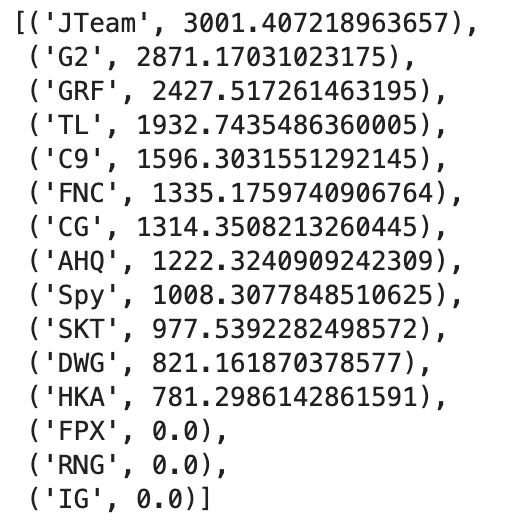
\includegraphics[width=2in]{TeamRanking}
	\end{center}
	We see an LMS team ranked at the top, which has never happened in the history of World's. However, it is actually easily explainable why the scores appear as they do. In the LMS, when J Team won, they were either huge blowouts or close. Which is the case for a lot of regions that aren't the LCK and LPL. There are usually those $1$ to $2$ teams per region that just stomps their opponents. However, this inflates our overall results when trying to compare those regions with much more competiive regions. The true outlier is Griffin in the LCK. Griffin was the greatest best of 1 team the LCK has seen in years, not only did they have the best summer split record, but they destroyed their opponents by a large margin whenever they won. The LPL scores are zero, because there is that much missing LPL data unfortunately. The VCS doesn't have data collected for it either, but they are a non-factor when trying to predict world's anyway, so not a big deal. Now if we replace each team on this list by region with their seed number, we get,
	\begin{center}
		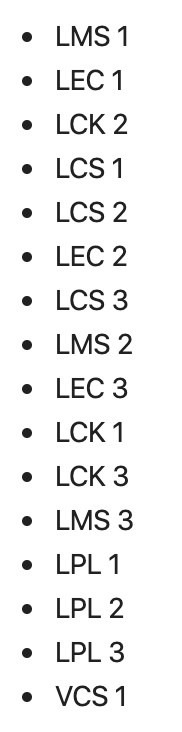
\includegraphics[width=.75in]{RegionRanking}
	\end{center}
	
	In the history of League of Legends this has never happened. Thus, using this as a predictor on its own is not a good choice. This Linear Model may be much more effective to predict the knockout stage, and region influence will be a lot less valued. However, if we reorder this list based off past World's results with group stages while keeping the order in which teams appear per region, then we get,
	\begin{center}
		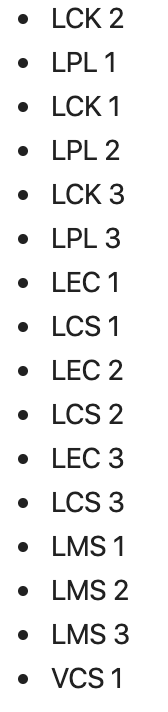
\includegraphics[width=.75in]{CorrectedRR}
	\end{center}
	
	This result is not only much more believable, but if applied to past group stages at World's, then it gets a near perfect for every group stage. The problem with this approach, is that even though we boosted the accuracy a ton, we miss out on catching upsets.
\section{Knockout Stage}	
	The knockout stage is the quaterfinals, semifinals, and finals of the world championships. It consists the 1st and 2nd seeds from each group randomly drawn into the bracket, except two teams from the same group cannot be on the same side of the bracket.

\subsection{Midseason Invitational}
	In the beginning the midseason invitational (MSI) was mentioned. This should probably be used somehow with predicting the knockout stage, since it is the one time teams met internationally and played best of 5's. When it came to group stage, MSI didn't make a difference. If anything it boosted the idea to have the region power ranking reorder even more.
	
	
	It matters for the knockout stage, because it could give insight on predicting how the last part of the world's bracket plays out. However, we only want to use the results, since it happened right before summer split and a lot can change over the course of a whole split. The only matches from 2019 MSI that could matter for 2019 World's is Team Liquid vs Invictus Gaming and G2 Esports vs SKT Telecom T1. That showed $\text{LEC} > \text{LCK}$ in the best of five, and $\text{LCS} > \text{LPL}$ in the best of five. It also showed G2 beating Team Liquid in the final or $\text{LEC} > \text{LCS}$. It did not show $\text{LEC} > \text{LPL}$, especially since the LPL team dominated the LEC team in the best of one stage at MSI.

\subsection{Group Stage Data}
	All summer split data used to determine group stage no longer matters. The region ranking system used to predict groups no longer matters. There were not that many games in the group stage to replace the amount of data we got from summer split, however, we have data for teams playing each other on the international stage now. Results from using the model and getting a new ranking.
	
	\begin{center}
		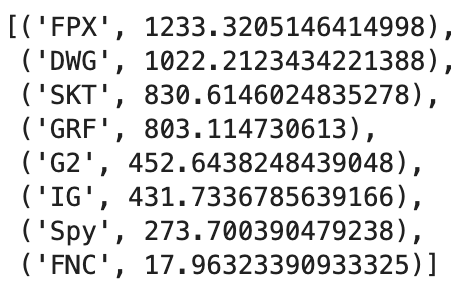
\includegraphics[width=1.5in]{BeforeSeed}
	\end{center}

\subsubsection{G2 Esports and IG Factor}
	The rating above is fantastic except for two major outliers. Those outliers are G2 and IG. G2 has never lost a best of five all season against. This includes MSI which they won, thus giving them seed priority as being a first seed for the region and for the tournament has to play-in somehow. Seeding them higher than FPX doesn't make sense since they are both the first seed from their region, but cheating them to be second place in the power rankings is a more suitable argument.
	
	
	Invictus Gaming or IG are the reigning world champions. Their performance was lackluster in group stage according to our ranking. It is hard to tell whether or not they should be cheated up in rank, because at MSI 2019 they also lost their best of five match against Team Liquid from the LCS.
	
	
	Overall, both of the teams at first glance seem like major outliers. Giving G2 benefit of the doubt that they will beat SKT and Damwon Gaming makes sense because they beat SKT convincingly at MSI, and SKT beat Damwon Gaming in the best of five during summer split. 
	
\subsection{Reflection}
	Outside of G2 being rated so low by the model, this linear model seems like a good overall predictor. FPX was the first seed from the LPL. The LCK teams all ranked very highly because the region itself is a very strong region, and statistically it shows. When predicting the 2019 knockout stage, we'll consider results with having G2 below FPX, and G2 placed where it is.
	

\section{Predicting 2019}
	The 2019 world championships have already happened this year and the team Funplus Phoenix from the LPL won. They were led by their midlaner Doinb, and their jungler Tian was awarded MVP. Thus, the linear algebra we are using to get the result is technically being tweaked using results that have already happened. However, all the matches that have to deal with the quarterfinals and up were removed from the data before creating the "rankings" with the model. The world's data was not used for predicting the group stage at all, as the play-in stage data is irrelevant to the group stage data.
	
	
	If we apply the results from the group stage section after we reorder by region we get,
	\begin{center}
		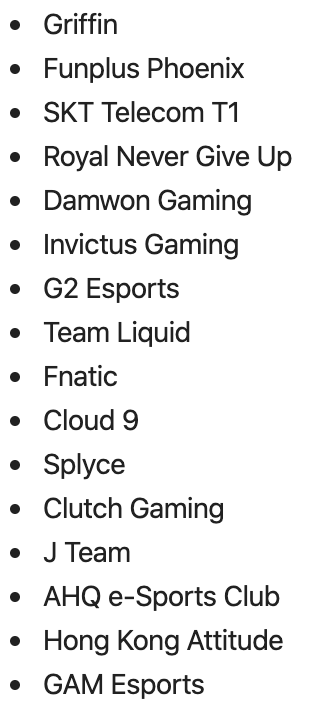
\includegraphics[width=.75in]{Ranking}
	\end{center}
	 
	 Below are my picks I made for the World's group stage with a lot of bias for North America LCS because I just wanted to see them win. The left side of each group is how I seeded them, and the right side of each group is the seed they got.
	 
	 \begin{center}
	 	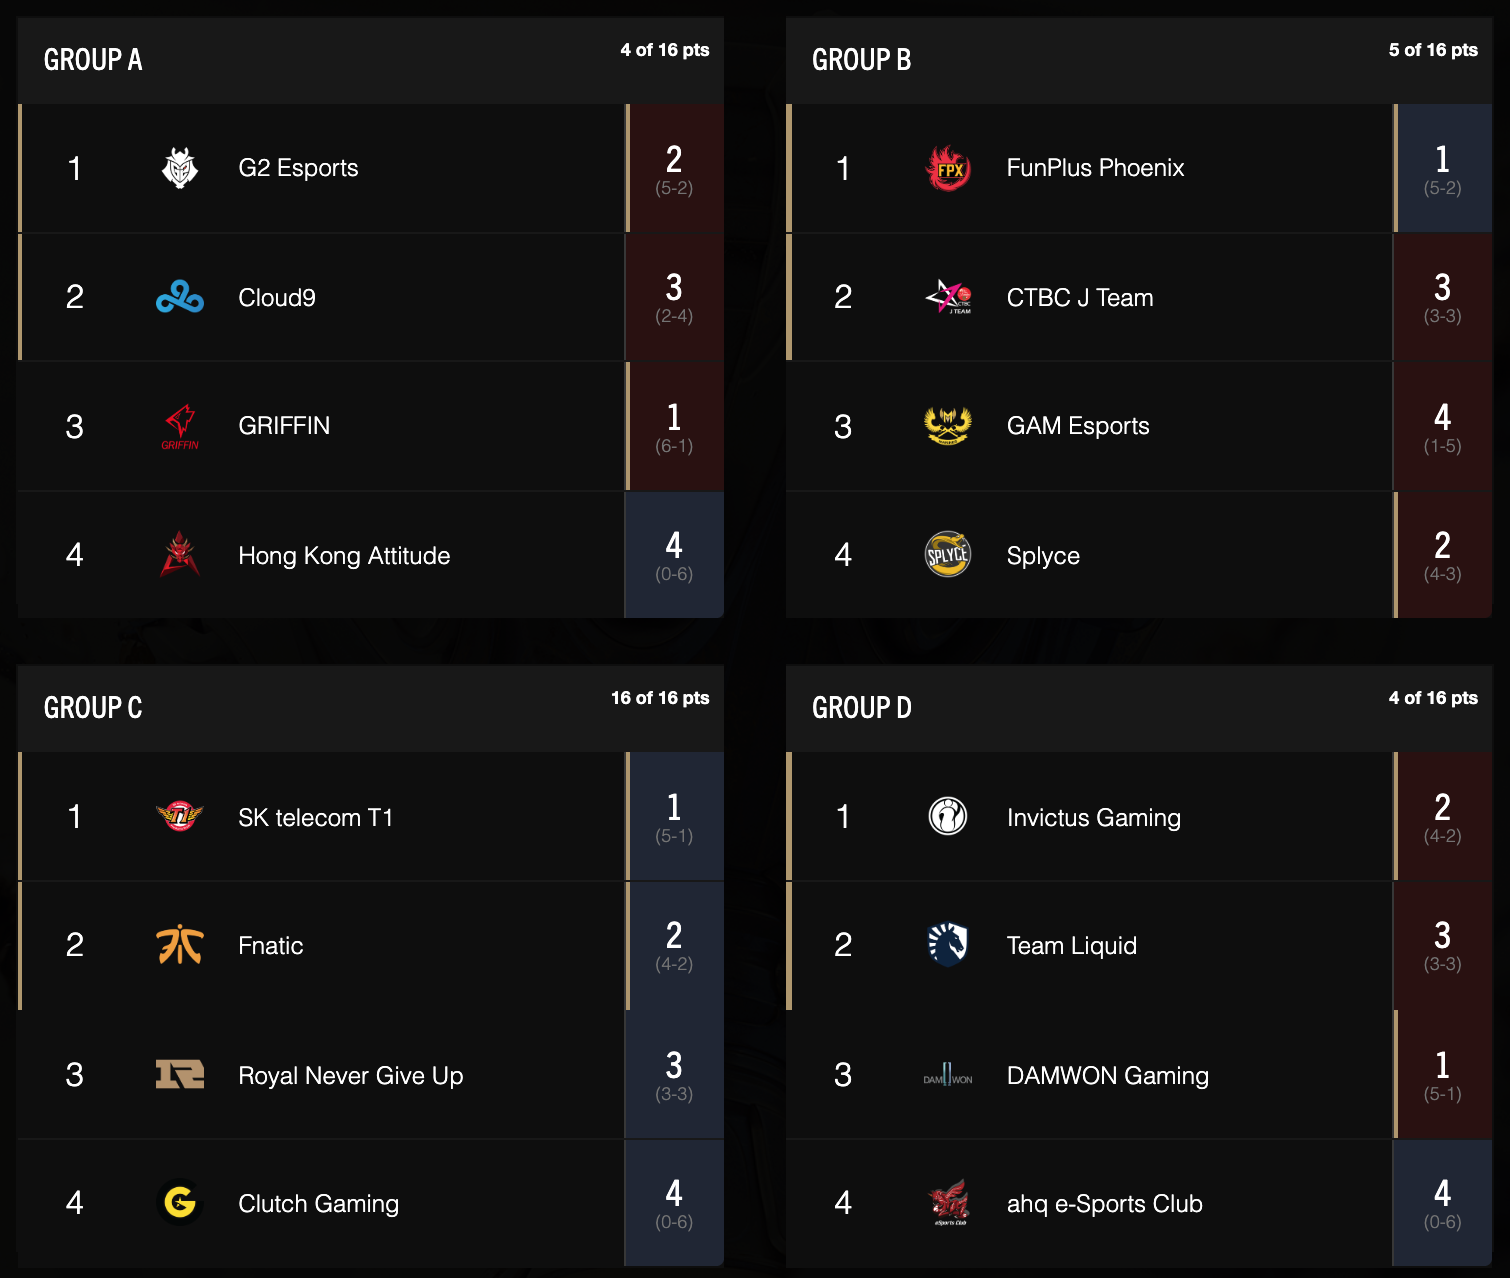
\includegraphics[width=2in]{MyPicks}
	 \end{center}
 
 	If we use the ranking we got from the group stage section and apply it to this image. The only rating we get wrong is picking Royal Never Give Up to outplace Fnatic in Group C. Otherwise, every group would end up getting rated correctly. Fnatic beating out Royal Never Give Up for the second seed was also considered an upset by many League of Legends analysis that didn't have a bias for the LEC.
 	
 	
 	The results from the 2019 knockout stage are as follows, 
 	\begin{center}
 		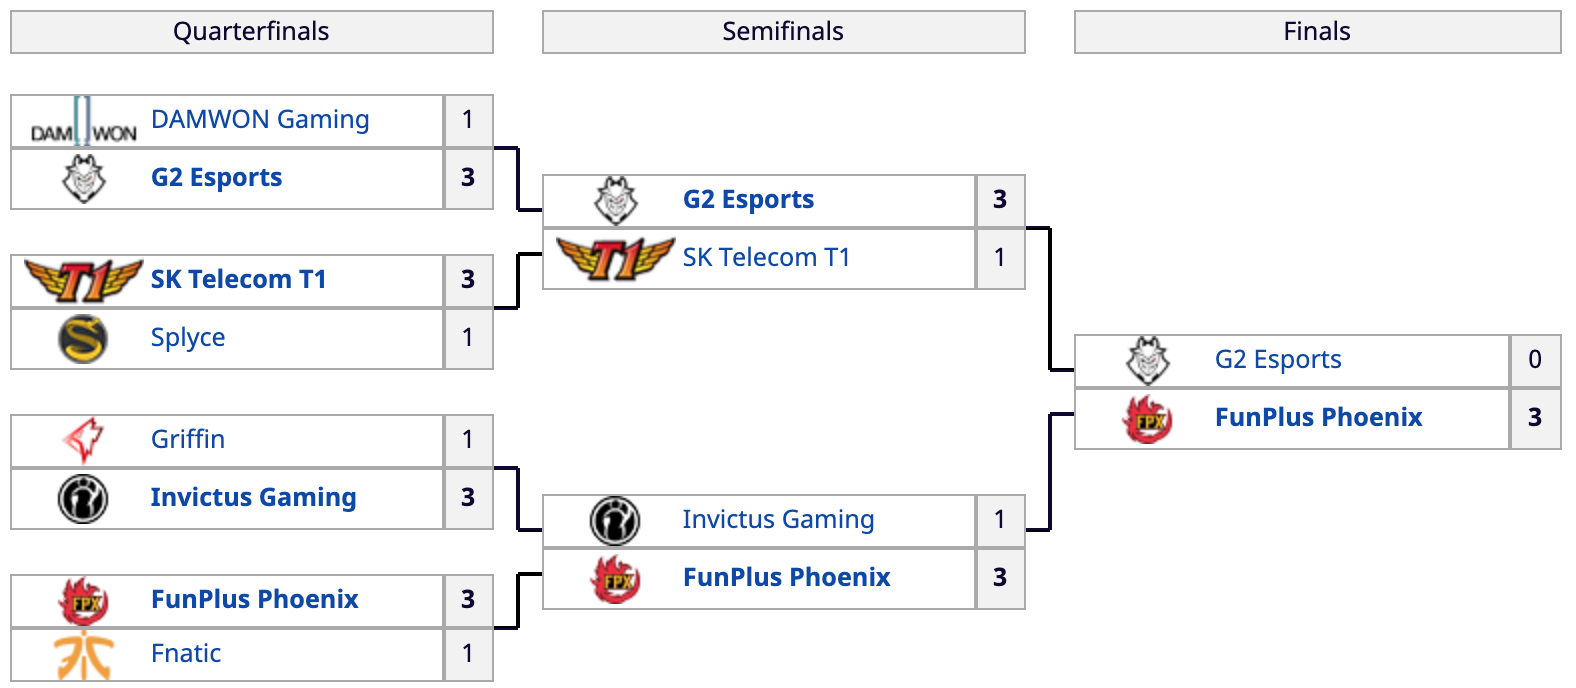
\includegraphics[width=3in]{Knockout}
 	\end{center}
 	
 	As can be seen if we acknowledge that our model had G2 as a severe outlier and rank it below FPX because they were both first seeds from their region, then we only get the quarterfinal match between IG and Griffin incorrect. If we do not acknowledge the chance that G2 was a sever outlier on the ranking, then we get the IG vs Griffin game and the G2 side of the bracket incorrect.

\section{Conclusion}
	This project turned out to be a semi-supervised project. League of Legends doesn't appear to be a developed enough game unfortunately to predict like NCAA march madness is. It is unfortunate how much region bias matters with this project. If we look at past world's results, and base our bracket predictions based off our model and slight region reordering we get a near perfect group stage. Picking G2 to be second seed in our power ranking after groups only because they won MSI is an unfortunate outcome as well. It seems the best way to use machine learning to predict the world's bracket is as a loose guide to gain a power ranking for individual regions in for the group stage part. For the knockout stage, the model was surprisingly accurate.
	
	
	After watching the matches over from the knockout stage and group stage from world's there was one noticeable thing in this sport that most sports don't have. If a major teamfight happened towards the end of the game, then the person who was winning the whole time would end up losing. Catching variance like that seems really challenging. Exploring ways to catch that variance would be an angle worth approaching.




\begin{thebibliography}{1}
			\bibitem{1st} Svenhuysen, Tim {\em Oracle's Elixir} Oracle's Elixir, 2015. Web
			$<$\href{http://oracleselixir.com/about/}{Website for Oracle's Elixir} $>$
			\bibitem{2nd} Gamepedia. Web.
				$<$Website that is mainly filled in by fans. Trusted website for having consistent data about history with competitive gaming and other similar topics. \href{https://lol.gamepedia.com/League_of_Legends_Esports_Wiki}{Website for Gamepedia}$>$
			\bibitem{3rd} My Pick'em, 2019. Web.
				$<$Created when I entered the pick'em challenge for World's 2019. \href{http://pickem.lolesports.com/share/series/6/user/2482088/my-picks}{Website for my Pick'em}$>$
			\bibitem{4th} Esportpedia. Web.
			$<$Website that is mainly filled in by fans. Trusted website for having consistent data about history with e-sports. Often has more reliable graphics then gamepedia. \href{https://www.esportspedia.com/lol/Worlds_Main_Event_2019}{Website for Esportspedia}$>$
\end{thebibliography}

	
	
	
	
	
 
\end{document}

